\chapter{Facelets}

	Dieses Kapitel enthält alle benötigten  Facelets. Jedes Facelet wird in unterschiedliche  Bereiche aufgeteilt:
	\begin{itemize}
		\item \textbf{Beschreibung} beinhaltet die Funktionen des Facelets.
		\item \textbf{Links} enthält die Seiten, auf welche weitergeleitet wird.
		\item \textbf{Buttons} listet die sich auf der Seite befindlichen Buttons mit deren hinterlegten Methoden auf.
		\item \textbf{Inputs} enthält eine Liste aller Eingabefelder auf der Seite.
		\item \textbf{Outputs} enthält eine Liste aller Ausgabefelder auf der Seite.
		\item \textbf{Backing Bean} gibt das mit dem Facelet verbundene Bean an.
	\end{itemize}
	
	\section{Templates}
		Kathi, Ricky
		Das Standard-Template, an dem sich alle Facelets orientieren ist in Abbildung 4.1 zu sehen. Hier wird in drei Teilbereiche unterschieden. Es gibt den Teilbereich \glqq Header\grqq\, welcher hauptsächlich die von der Benutzerrolle abhängige Navigation (\hyperlink{navigation}{navigation.xhtml}) beinhaltet, den Teilbereich \glqq Content\grqq\, welcher abhängig vom jeweils aufgerufenen Facelet befüllt wird und den Teilbereich \glqq Footer\grqq\, welcher den unteren Bereich der dargestellten Seite befüllt (\hyperlink{footer}{footer.xhtml}).

			\begin{figure}[h]
				\centering
				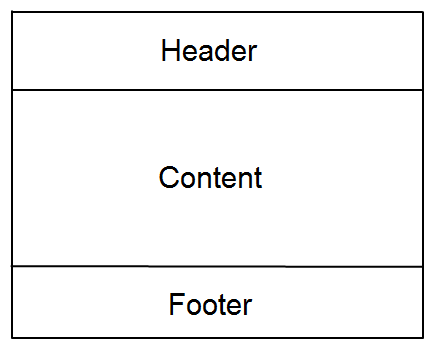
\includegraphics[width=0.3\textwidth]{Grafiken/Template.png}
	  			\caption{Standard-Template für alle Facelets}
			\end{figure}
			
		\paragraph{navigation.xhtml} \hypertarget{navigation}
			RS\\
			\begin{itemize}
				\item \textbf{Beschreibung:} Hier kann, abhängig von der Benutzerrolle, durch die Seite navigiert werden.
				\item \textbf{Links:}
					\begin{itemize}
						\item Suche: Navigiert zur Kurse durchsuchen Seite. 
						\item Sprache Deutsch: Ändert die angezeigte Sprache zu Deutsch.
						\item Sprache Englisch: Ändert die angezeigte Sprache zu Englisch.
						\item Profil (Benutzer): Navigiert zum eigenen Profil.
						\item Meine Kurse (Benutzer): Navigiert zur Anzeige der eigenen Kurse.
						\item Terminplaner (Benutzer): Navigiert zum persönlichen Terminplaner.
						\item Seitenverwaltung (Administrator): Lässt den Seitenadministrator zur Seitenverwaltung navigieren.
						\item Benutzer aktivieren: (Kursleiter, Administrator): Navigiert zur Benutzer aktivieren Seite.
					\end{itemize}
				\item \textbf{Buttons:}
					\begin{itemize}
						\item Logout (Benutzer, wenn eingeloggt): Loggt den aktuellen eingeloggten Benutzer aus. \\ Zugehörige Methode: logout()
						\item Anmelden (Anonym): Navigiert zur Registrierungs- und Anmeldeseite. \\ Zugehörige Methode: login()
					\end{itemize}
				\item \textbf{Inputs:} -
				\item \textbf{Outputs:}
					\begin{itemize}
						\item Logo: Zeigt verkleinertes, vom Administrator definiertes Logo der Website. Beim klick gelangt der Nutzer zur \hyperlink{index}{Startseite}.
					\end{itemize}
				\item \textbf{BackingBean:}
					\begin{itemize}
						\item Navigation.java
					\end{itemize}
			\end{itemize}

		\paragraph{footer.xhtml} \hypertarget{footer}
			RS\\
			\begin{itemize}
				\item \textbf{Beschreibung:} Dieses Facelet dient der Darstellung des Footers.
				\item \textbf{Links:} -
				\item \textbf{Buttons:}
					\begin{itemize}
						\item AGB: Navigiert zum Facelet mit den Allgemeinen Geschäftsbedingungen. Zugehörige Methode: loadAGBPage()
						\item Impressum: Navigiert zum Facelet mit dem Impressum der Webanwendung. Zugehörige Methode: loadImprintPage()
						\item Hilfe: Navigiert zur Hilfeseite. Zugehörige Methode: loadHelpPage()
					\end{itemize}
				\item \textbf{Inputs:} -
				\item \textbf{Outputs:} -
				\item \textbf{BackingBean:}
					\begin{itemize}
						\item Footer.java
					\end{itemize}
			\end{itemize}
	
	\section{Facelets}
	
		\subsection{open}
			
			\subsubsection{common}
			
				\paragraph{index.xhtml} \hypertarget{index}
					RS\\
					\begin{itemize}
						\item \textbf{Beschreibung:} Dieses Facelet stellt die Startseite des Systems dar.
						\item \textbf{Links:}
							\begin{itemize}
								\item Gesamtes Kursangebot, \hyperlink{search}{search.xhtml}
							\end{itemize}
						\item \textbf{Buttons:} -
						\item \textbf{Inputs:} -
						\item \textbf{Outputs:}
							\begin{itemize}
								\item Logo der Website
							\end{itemize}
						\item \textbf{BackingBean:} -
					\end{itemize}
				
				\paragraph{authenticate.xhtml} \hypertarget{authenticate}
				KH\\
				\begin{itemize}
					\item \textbf{Beschreibung:}
					Auf dieser Seite kann man sich im System anmelden, ein neues Benutzerkonto generieren oder ein neues Passwort anfordern.
					\item \textbf{Links:} -
					\item \textbf{Buttons:}
						\begin{itemize}
							\item Registrieren: Durch Drücken dieses Buttons wird der neue Benutzer mit den eingegebenen Daten im System gespeichert und es wird eine Bestätigungsmail mit dem Verifizierungslink an die angegebene E-Mail-Adresse verschickt, sofern alle Daten korrekt eingegeben wurden. \\ Zugehörige Methode: registerUser()
							\item Anmelden: Durch Drücken dieses Buttons wird der registrierte Benutzer im System angemeldet und auf die Seite 'Meine Kurse' (\hyperlink{myCourses}{myCourses.xhtml}) weitergeleitet, sofern Benutzername und Passwort korrekt eingegeben wurden. \\ Zugehörige Methode: login()
							\item Passwort vergessen: Durch Drücken dieses Buttons wird an die angegebene E-Mail-Adresse ein automatisch generiertes Passwort geschickt, sofern die Adresse im System existiert. \\ Zugehörige Methode: resetPassword()
						\end{itemize}
					\item \textbf{Inputs:}
						\begin{itemize}
							\item Anrede (Registrierung): Hier wählt der Benutzer die Anrede 'Herr' oder 'Frau' aus.
							\item Vorname (Registrierung): Hier trägt der Benutzer seinen Vornamen ein.
							\item Name (Registrierung): Hier gibt der Benutzer seinen Namen ein.
							\item Benutzername (Registrierung): Hier gibt der Benutzer einen Benutzernamen ein.
							\item Passwort (Registrierung): Hier trägt der Benutzer ein Passwort ein.
							\item Passwort bestätigen (Registrierung): Hier gibt der Benutzer das gleiche Passwort erneut ein zur Bestätigung.
							\item Geburtstag (Registrierung): Hier gibt der Benutzer sein Geburtsdatum ein.
							\item Straße/Hausnummer (Registrierung): Hier gibt der Benutzer seine Straße und seine Hausnummer ein.
							\item Stadt (Registrierung): Hier trägt der Benutzer seine Stadt ein.
							\item Postleitzahl (Registrierung): Hier trägt der Benutzer seine Postleitzahl ein.
							\item Land (Registrierung): Hier trägt der Benutzer sein Heimatland ein.
							\item E-Mail-Adresse (Registrierung): Hier gibt der Benutzer seine E-Mail-Adresse ein.
							\item AGBs bestätigen (Registrierung): Durch Setzten des Häkchens bestätigt der Benutzer die AGBs. 
							\item Benutzername (Anmeldung): Der Benutzer gibt seinen Benutzernamen ein, mit dem er sich registriert hat.
							\item Passwort (Anmeldung): Der Benutzer gibt sein Passwort ein, mit dem er sich registriert hat.
							\item E-Mail-Adresse (Passwort vergessen): Der Benutzer gibt seine im System bereits gespeicherte E-Mailadresse ein.
						\end{itemize}
					\item \textbf{Outputs:} 
						\begin{itemize}
							\item Vorname Fehlermeldung (Registrierung): Ausgabe der Fehlermeldungen zu den Validatoren des Eingabefeldes.
							\item Name Fehlermeldung (Registrierung): Ausgabe der Fehlermeldungen zu den Validatoren des Eingabefeldes.
							\item Benutzername Fehlermeldung (Registrierung): Ausgabe der Fehlermeldungen zu den Validatoren des Eingabefeldes.
							\item Passwort Fehlermeldung (Registrierung): Ausgabe der Fehlermeldungen zu den Validatoren des Eingabefeldes.
							\item Passwort bestätigen Fehlermeldung (Registrierung): Ausgabe der Fehlermeldungen zu den Validatoren des Eingabefeldes.
							\item Geburtstag Fehlermeldung (Registrierung): Ausgabe der Fehlermeldungen zu den Validatoren des Eingabefeldes.
							\item Straße/Hausnummer Fehlermeldung (Registrierung): Ausgabe der Fehlermeldungen zu den Validatoren des Eingabefeldes.
							\item Stadt Fehlermeldung (Registrierung): Ausgabe der Fehlermeldungen zu den Validatoren des Eingabefeldes.
							\item Postleitzahl Fehlermeldung (Registrierung): Ausgabe der Fehlermeldungen zu den Validatoren des Eingabefeldes.
							\item Land Fehlermeldung (Registrierung): Ausgabe der Fehlermeldungen zu den Validatoren des Eingabefeldes.
							\item E-Mail-Adresse Fehlermeldung (Registrierung): Ausgabe der Fehlermeldungen zu den Validatoren des Eingabefeldes.
							\item AGBs bestätigen Fehlermeldung (Registrierung): Ausgabe der Fehlermeldungen zu den Validatoren des Eingabefeldes.
							\item Benutzername Fehlermeldung (Anmeldung): Ausgabe der Fehlermeldungen zu den Validatoren des Eingabefeldes.
							\item Passwort Fehlermeldung (Anmeldung): Ausgabe der Fehlermeldungen zu den Validatoren des Eingabefeldes.
							\item E-Mail-Adresse Fehlermeldung (Passwort vergessen): Ausgabe der Fehlermeldungen zu den Validatoren des Eingabefeldes.
						\end{itemize}
					\item \textbf{BackingBean:}
						\begin{itemize}
							\item AuthenticateUser.java
							\item RegisterUser.java
							\item LostPassword.java
						\end{itemize}
				\end{itemize}
				
				\paragraph{imprint.xhtml} \hypertarget{imprint}
					KH\\
					\begin{itemize}
						\item \textbf{Beschreibung:} Auf dieser Seite kann das Impressum angezeigt werden.
						\item \textbf{Links:} -
						\item \textbf{Buttons:} -
						\item \textbf{Inputs:} -
						\item \textbf{Outputs:} 
							\begin{itemize}
								\item	Anzeige des Impressums, welches vom Administrator festgelegt wurde.
							\end{itemize}
						\item \textbf{BackingBean:} -
					\end{itemize}
				
				\paragraph{agb.xhtml} \hypertarget{agb}
					RS\\
					\begin{itemize}
						\item \textbf{Beschreibung:} Dieses Facelet dient der Anzeige der Allgemeinen Geschäftsbedingungen.
						\item \textbf{Links:} -
						\item \textbf{Buttons:} -
						\item \textbf{Inputs:} -
						\item \textbf{Outputs:}
							\begin{itemize}
								\item von Betreibern festgelegte Allgemeine Geschäftsbedingungen.
							\end{itemize}
						\item \textbf{BackingBean:} -
					\end{itemize}

		
			\subsubsection{courses}
				
				\paragraph{search.xhtml} \hypertarget{search}
					RS\\
					\begin{itemize}
						\item \textbf{Beschreibung:} Hier können alle Kurse angezeigt und durchsucht werden.
						\item \textbf{Links:} -
						\item \textbf{Buttons:}
							\begin{itemize}
								\item Anzeigen: Zeigt die Angebote im ausgewählten Zeitraum an. \\ Zugehörige Methode: displayCoursesInSpecificPeriod()
								\item Suchen: Durchsucht die Website nach dem eingegebenen Suchbegriff mittels gewählten Suchobjekt. \\ Zugehörige Methode: search()
							\end{itemize}
						\item \textbf{Inputs:}
							\begin{itemize}
								\item Angebotszeitraum: Ermöglicht eine genauere Anzeige des Kursangebots, entweder Tagesangebot, Wochenangebot oder das gesamte Angebot. Die detaillierteren Suchoptionen sind nur für registrierte Benutzer verfügbar.
								\item Suchobjekt (abhängig von Benutzerrolle): Ermöglicht eine genauere Suche, beispielsweise nach Kursen, Kursleitern oder Kurs-ID.
							\end{itemize}
						\item \textbf{Outputs:}
							\begin{itemize}
								\item Tabelle mit Ergebnissen der Suche.
								\item Schaltfläche um zwischen Ergebnissen zu Blättern.
							\end{itemize}
						\item \textbf{BackingBean:}
							\begin{itemize}
								\item SearchCourse.java
							\end{itemize}
					\end{itemize}
				
				\paragraph{courseDetails.xhtml} \hypertarget{courseDetails}
					RS\\
					\begin{itemize}
						\item \textbf{Beschreibung:} Zur genaueren Betrachtung eines einzelnen Kurses wird dieses Facelet benötigt.
						\item \textbf{Links:} -
						\item \textbf{Buttons:}
							\begin{itemize}
								\item Anmelden (Benutzer, noch nicht angemeldet): Meldet den Benutzer zum Kurs an. \\ Zugehörige Methode: signUpForCourse()
								\item Abmelden (Benutzer, wenn angemeldet): Meldet den Benutzer vom Kurs ab. \\ Zugehörige Methode: signOffFromCourse()
								\item Teilnehmer anzeigen (Kursleiter): Zeigt die zum Kurs angemeldeten Benutzer an. \\ Zugehörige Methode: loadParticipantsPage()
								\item Alle auswählen (Benutzer, zum Kurs angemeldet): Wählt alle Kurseinheiten des Kurses aus. \\ Zugehörige Methode: selectAllCourseUnits()
								\item Speichern (Benutzer, zum Kurs angemeldet): Speichert alle ausgewählten Kurseinheiten und meldet den Nutzer dazu an. \\ Zugehörige Methode: signUpForCourseUnits()
								\item Bearbeiten (Administrator, noch nicht im Bearbeitungsmodus): Ermöglicht die Bearbeitung der einzelnen Kursdetails. \\ Zugehörige Methode: editCourse()
								\item Speichern (Administrator, im Bearbeitungsmodus): Speichert alle vorgenommenen Kursänderungen. \\ Zugehörige Methode: saveCourse()
								\item Hinzufügen (Administrator): Fügt einen Kursleiter zum Kurs hinzu. Zugehörige Methode: addCourseLeader()
								\item Kurseinheit anlegen (Kursleiter): Erstellt eine neue Kurseinheit zum Kurs. \\ Zugehörige Methode: loadCreateCourseUnitPage()
								\item Kurseinheit bearbeiten (Kursleiter): Ermöglicht die Bearbeitung einer einzelnen Kurseinheit. \\ Zugehörige Methode: loadEditCourseUnitPage()
								\item Kurs löschen (Administrator): Löscht den Kurs. \\ Zugehörige Methode: deleteCourse()
							\end{itemize}
						\item \textbf{Inputs:}
							\begin{itemize}
								\item Kursnews erhalten: Trägt Benutzer bei Anmeldung zum Kurs in die Kursnews ein.
								\item Kurseinheit auswählen: Wählt Kurseinheit aus, zu der sich der Nutzer anmelden möchte.
								\item Kursleiter auswählen (Administrator): Wählt Kursleiter aus, welcher gelöscht werden soll.
								\item Kursleiter Name (Administrator): Eingabefeld für den Namen eines neuen Kursleiters.
								\item Kursleiter E-Mail (Administrator): Eingabefeld für die E-Mail Adresse eines neuen Kursleiters.
								\item Kursbeschreibung (Administrator): Eingabefeld für die Kursbeschreibung.
								\item Minimale Teilnehmerzahl (Administrator): Eingabefeld für die minimale Teilnehmerzahl des Kurses.
								\item Maximale Teilnehmerzahl (Administrator): Eingabefeld für die maximale Teilnehmerzahl des Kurses.
								\item Startdatum (Administrator): Eingabefeld für das Startdatum des Kurses.
								\item Enddatum (Administrator): Eingabefeld für das Enddatum des Kurses.
							\end{itemize}
						\item \textbf{Outputs:}
							\begin{itemize}
								\item Tabelle Kursleiter: Tabelle mit den Kontaktinformationen der/des Kursleiters.
								\item Tabelle Kurseinheiten: Tabelle mit allen Kurseinheiten des Kurses und zugehörigen Informationen wie Ort, Preis oder Datum.
								\item Kurs-ID: Zeigt die zum Kurs zugehörige ID an.
								\item Kursbeschreibung: Zeigt die Beschreibung zum Kurs an.
								\item Minimale Teilnehmerzahl: Zeigt die für den Kurs minimale Teilnehmerzahl an.
								\item Maximale Teilnehmerzahl: Zeigt die für den Kurs maximale Teilnehmerzahl an.
								\item Fehlermeldung zu den einzelnen Eingabefeldern, bei falscher Eingabe.
							\end{itemize}
						\item \textbf{BackingBean:}
							\begin{itemize}
								\item CourseDetail.java
								\item CourseManagement.java
							\end{itemize}
					\end{itemize}
		
		\subsection{users}
		
			\subsubsection{registeredUser}
				
				\paragraph{myCourses.xhtml} \hypertarget{myCourses}
					KH\\
					\begin{itemize}
						\item \textbf{Beschreibung:} Auf dieser Seite werden alle Kurse angezeigt, in die der Teilnehmer eingetragen ist.
						\item \textbf{Links:}
							\begin{itemize}
								\item Kurstitel: Über die Kurstitel gelangt der Benutzer auf die jeweilige Kursdetailseite. (\hyperlink{courseDetails}{courseDetails.xhtml})
							\end{itemize}
						\item \textbf{Buttons:} -
						\item \textbf{Inputs:} -
						\item \textbf{Outputs:}
							\begin{itemize}
								\item Tabelle Auflistung aller Kurse: Hier werden dem Benutzer alle seine angemeldeten Kurse angezeigt.
							\end{itemize}
						\item \textbf{BackingBean:}
							\begin{itemize}
								\item MyCourses.java
							\end{itemize}
					\end{itemize}
				
				\paragraph{profile.xhtml} \hypertarget{profile}
					KH\\
					\begin{itemize}
						\item \textbf{Beschreibung:} Auf dieser Seite werden die persönlichen Daten und der Kontostand des Benutzers angezeigt. Der Benutzer kann die Daten ändern und sein Konto aufladen. Der Kursleiter kann hier den Benutzer aktivieren, und der Administrator den Benutzer löschen.
						\item \textbf{Links:} -
						\item \textbf{Buttons:}
							\begin{itemize}
								\item Bearbeiten: Nach Klicken auf diesen Button können die persönlichen Daten geändert werden. Der Button trägt nun die Aufschrift 'Speichern' und ist mit dessen dazugehöriger Methode hinterlegt. \\ Zugehörige Methode: editUserData()
								\item Speichern: Durch Drücken dieses Buttons werden die vorgenommenen Änderungen gespeichert, sofern alle Daten korrekt eingegeben wurden. Bei Änderung der E-Mail-Adresse wird außerdem eine Bestätigungsmail mit einem Verifizierungslink verschickt. Bei erfolgreicher Speicherung erscheint der Button 'Bearbeiten' anstelle des Button 'Speichern'. \\ Zugehörige Methode: saveUserData()
								\item Durchsuchen: Durch Drücken dieses Buttons kann das eigene Dateiverzeichnis nach einem Bild durchsucht werden.
								\item Hochladen: Durch Drücken dieses Buttons wird das ausgewählte Profilbild hochgeladen. \\ Zugehörige Methode: uploadProfilPic()
								\item Konto aufladen: Durch Klicken dieses Buttons wird der Benutzer auf die Seite 'Kontoaufladung' (\hyperlink{buyCredits}{buyCredits.xhtml})  weitergeleitet. \\ Zugehörige Methode: depositMoneyPerCreditCard()
								\item Benutzer löschen: Durch Drücken dieses Buttons entfernt der Administrator diesen Benutzer aus dem System, oder der Benutzer kann sich selbst auf inaktiv setzen. \\ Zugehörige Methoden: deleteUser(), setUserInactive() 
							\end{itemize}
						\item \textbf{Inputs:}
							\begin{itemize}
								\item Vorname: Hier kann der Benutzer seinen Vornamen ändern.
								\item Name: Hier kann der Benutzer seinen Namen ändern.
								\item Geburtstag: Hier kann der Benutzer sein Geburtsdatum ändern.
								\item Straße/Hausnummer: Hier kann der Benutzer seine Straße und Hausnummer ändern.
								\item Stadt: Hier kann der Benutzer seine Stadt ändern.
								\item Postleitzahl: Hier kann der Benutzer seine Postleitzahl ändern.
								\item Land: Hier kann der Benutzer seine Land ändern.
								\item E-Mail-Adresse: Hier kann der Benutzer seine E-Mail-Adresse ändern.
								\item Benutzername: Hier kann der Benutzer seinen Benutzernamen ändern.
								\item Passwort: Hier kann der Benutzer sein Passwort ändern.
								\item Passwort bestätigen: Hier muss der Benutzer sein geändertes Passwort bestätigen.
								\item Benutzerrolle: Hier kann der Administrator die Benutzerrolle eines Nutzers ändern.
								\item Profilbild: Hier kann der Benutzer sein Profilbild ändern.
							\end{itemize}
						\item \textbf{Outputs:}
							\begin{itemize}
								\item Benutzer-ID: Ausgabe der automatisch generierten ID.
								\item Vorname Fehlermeldung: Ausgabe der Fehlermeldungen zu den Validatoren des Eingabefeldes.
								\item Name Fehlermeldung: Ausgabe der Fehlermeldungen zu den Validatoren des Eingabefeldes.
								\item Geburtstag Fehlermeldung: Ausgabe der Fehlermeldungen zu den Validatoren des Eingabefeldes.
								\item Straße/Hausnummer Fehlermeldung: Ausgabe der Fehlermeldungen zu den Validatoren des Eingabefeldes.
								\item Stadt Fehlermeldung: Ausgabe der Fehlermeldungen zu den Validatoren des Eingabefeldes.
								\item Postleitzahl Fehlermeldung: Ausgabe der Fehlermeldungen zu den Validatoren des Eingabefeldes.
								\item Land Fehlermeldung: Ausgabe der Fehlermeldungen zu den Validatoren des Eingabefeldes.
								\item E-Mail-Adresse Fehlermeldung: Ausgabe der Fehlermeldungen zu den Validatoren des Eingabefeldes.
								\item Benutzername Fehlermeldung: Ausgabe der Fehlermeldungen zu den Validatoren des Eingabefeldes.
								\item Passwort Fehlermeldung: Ausgabe der Fehlermeldungen zu den Validatoren des Eingabefeldes.
								\item Passwort bestätigen Fehlermeldung: Ausgabe der Fehlermeldungen zu den Validatoren des Eingabefeldes.
								\item Profilbild Fehlermeldung: Ausgabe der Fehlermeldungen zu den Validatoren des Eingabefeldes.
								\item Kontostand: Ausgabe des aktuellen Kontostandes.
								\item Tabelle Auflistung der Trainingskurse: Hier werden dem Kursleiter alle Kurse aufgelistet, die er leitet.
							\end{itemize}
						\item \textbf{BackingBean:}
							\begin{itemize}
								\item UserProfile.java
								\item UserManagement.java				
							\end{itemize}
					\end{itemize}
				
				\paragraph{buyCredits.xhtml} \hypertarget{buyCredits}
					RS\\
					\begin{itemize}
						\item \textbf{Beschreibung:} Hier kann der Nutzer mittels Kreditkarte seinen systeminternen Kontostand erhöhen.
						\item \textbf{Links:} -
						\item \textbf{Buttons:}
							\begin{itemize}
								\item Konto aufladen: Führt die Kontoaufladung aus. \\ Zugehörige Methode: depositAmount()
							\end{itemize}
						\item \textbf{Inputs:}
							\begin{itemize}
								\item CVC-Nummer: Prüfnummer der Kreditkarte.
								\item Ablaufdatum: Ablaufdatum der Kreditkarte.
								\item Nachname: Nachname des Nutzers zur Kontoaufladung.
								\item Vorname: Vorname des Nutzers zur Kontoaufladung.
								\item Kreditinstitut: Name des Kreditinstitutes des Nutzers zur Kontoaufladung.
								\item Kreditkartennummer: Nummer der Kreditkarte des Nutzers zur Kontoaufladung.
								\item Betrag: Geldbetrag, welcher auf das systeminterne Konto des Nutzers gebucht werden soll.
							\end{itemize}
						\item \textbf{Outputs:}
							\begin{itemize}
								\item Fehlermeldung zu den einzelnen Eingabefeldern, bei falscher Eingabe.
								\item Bestätigungsmeldung bei erfolgreicher Aufladung des Kontos.
							\end{itemize}
						\item \textbf{BackingBean:}
							\begin{itemize}
								\item PayementOnline.java
							\end{itemize}
					\end{itemize}
				
				\paragraph{scheduler.xhtml} \hypertarget{scheduler}
					RS\\
					\begin{itemize}
						\item \textbf{Beschreibung:} Persönlicher Terminplaner mit anstehenden Kursen.
						\item \textbf{Links:}
							\begin{itemize}
								\item Wochenansicht vorwärts: Zeigt die Termine der nächsten Woche an.
								\item Wochenansicht rückwärts: Zeigt die Termine der letzten Woche an.
							\end{itemize}
						\item \textbf{Buttons:} -
						\item \textbf{Inputs:} -
						\item \textbf{Outputs:}
							\begin{itemize}
								\item Wochentabelle: Zeigt von Montag bis Sonntag alle belegten Kurseinheiten an. Orientiert sich am klassischen Stundenplan, also mit stündlicher Ansicht.
							\end{itemize}
						\item \textbf{BackingBean:}
							\begin{itemize}
								\item Scheduler.java
							\end{itemize}
					\end{itemize}
				
				\paragraph{leaderProfile.xhtml} \hypertarget{leaderProfile}
					KH\\
					\begin{itemize}
						\item \textbf{Beschreibung:} Auf dieser Seite werden die Daten des Kursleiters, mit Ausnahme von sensiblen Daten wie Passwort oder Kontostand, und die von ihm geleiteten Kurse angezeigt.
						\item \textbf{Links:} -
						\item \textbf{Buttons:} -
						\item \textbf{Inputs:} -
						\item \textbf{Outputs:} 
							\begin{itemize}
								\item Tabelle Auflistung Kursleiterdaten: Hier werden die Daten des Kursleiters und die von ihm geleiteten Kurse angezeigt.
							\end{itemize}
						\item \textbf{BackingBean:}
						\begin{itemize}
							\item UserProfile.java			
						\end{itemize}
					\end{itemize}
				
				\paragraph{listParticipants.xhtml} \hypertarget{listParticipants}
					KH\\
					\begin{itemize}
						\item \textbf{Beschreibung:} Hier kann der registrierte Benutzer die Teilnehmer eines Kurses mit Benutzername und Profilbild ansehen. Dem Kursleiter werden zusätzlich die E-Mail-Adresse und die Information über den Erhalt von Kursnews angezeigt. Außerdem kann er einen Teilnehmer aus dem Kurs entfernen.
						\item \textbf{Links:} -
						\item \textbf{Buttons:}
							\begin{itemize}
								\item Löschen: Durch Drücken dieses Buttons kann der Kursleiter den entsprechenden Benutzer aus dem Kurs entfernen. \\ Zugehörige Methode: deleteUserFromCourse()
							\end{itemize}
						\item \textbf{Inputs:}
							 \begin{itemize}
							 	\item Entfernen: Durch Setzen des Häkchens wählt der Kursleiter diesen Benutzer aus, um ihn anschließend über den Button 'Löschen' zu entfernen.
							 \end{itemize}
						\item \textbf{Outputs:} 
							\begin{itemize}
								\item Tabelle Auflistung Kursteilnehmer: Hier werden die Teilnehmer des Kurses angezeigt.
							\end{itemize}
						\item \textbf{BackingBean:}
							\begin{itemize}
								\item ListParticipants.java
							\end{itemize}
					\end{itemize}
			
			\subsubsection{courseLeader}
			
				\paragraph{editCourseUnit.xhtml} \hypertarget{editCourseUnit}
					KH\\
					\begin{itemize}
						\item \textbf{Beschreibung:} Auf dieser Seite können Kursleiter beziehungsweise Administratoren Kurseinheiten anlegen und bearbeiten, oder Kursteilnehmer hinzufügen und entfernen
						\item \textbf{Links:} -
						\item \textbf{Buttons:}
							\begin{itemize}
								\item Bearbeiten (Kurseinheit): Nach Klicken auf diesen Button können die Daten der Kurseinheit geändert beziehungsweise eingetragen werden. Der Button trägt nun die Aufschrift 'Speichern' und ist mit dessen dazugehöriger Methode hinterlegt. \\ Zugehörige Methode: editCourseUnit()
								\item Speichern (Kurseinheit): Durch Drücken dieses Buttons werden die vorgenommenen Änderungen gespeichert, sofern alle Daten korrekt eingegeben wurden. Bei erfolgreicher Speicherung erscheint der Button 'Bearbeiten' anstelle des Button 'Speichern'. \\ Zugehörige Methode: saveCourseUnit()
								\item Löschen (Kurseinheit): Durch Drücken des Button 'Löschen' wird die Kurseinheit entfernt. \\ Zugehörige Methode: deleteCourseUnit()
								\item Löschen (Teilnehmer): Durch Drücken dieses Buttons wird der markierte Teilnehmer aus der Kurseinheit entfernt. \\ Zugehörige Methode: deleteUserFromCourseUnit()
								\item Hinzufügen (Teilnehmer): Durch Drücken dieses Buttons wird der angegebene Teilnehmer zu dieser Kurseinheit hinzugefügt, sofern der Benutzername im System existiert und die Daten korrekt eingegeben wurden. \\ Zugehörige Methode: addUserToCourseUnit()
							\end{itemize}
						\item \textbf{Inputs:}
							\begin{itemize}
								\item Termin: Hier gibt der Kursleiter den Termin der Kurseinheit ein.
								\item Straße/ Hausnummer: Hier gibt der Kursleiter Straße und Hausnummer ein.
								\item Postleitzahl: Hier gibt der Kursleiter die entsprechende Postleitzahl ein.
								\item Stadt: Hier gibt der Kursleiter die Stadt ein, in der die Kurseinheit stattfindet.
								\item Ort: Hier gibt der Kursleiter den Ort (Raumnummer, Turnhalle,..) ein, in dem die Kurseinheit stattfindet.
								\item Beschreibung: Hier gibt der Kursleiter die Beschreibung der Kurseinheit ein.
								\item Preis: Hier gibt der Kursleiter den Preis der Kurseinheit ein.
								\item Kursleiter: Hier wird der Leiter des Kurses angezeigt.
								\item Mindestteilnehmerzahl: Hier gibt der Kursleiter die minimale Teilnehmerzahl der Kurseinheit an.
								\item Maximale Teilnehmerzahl: Hier gibt der Kursleiter die maximale Teilnehmerzahl der Kurseinheit an.
								\item Teilnehmer markieren: Hier kann der Kursleiter einen Hacken setzen, um den Teilnehmer für das anschließende Löschen zu markieren.
								\item Benutzer-ID: Hier gibt der Kursleiter die Benutzer-ID des Teilnehmers an, welchen er zu der Kurseinheit hinzufügen will.
								\item Name (Teilnehmer): Hier gibt der Kursleiter den entsprechenden Namen des Teilnehmers an, welchen er zu der Kurseinheit hinzufügen will.
								\item Vorname (Teilnehmer): Hier gibt der Kursleiter den entsprechenden Vornamen des Teilnehmers an, welchen er zu der Kurseinheit hinzufügen will.
								\item Checkbox regelmäßig: Durch Setzen dieses Hackens markiert der Kursleiter den Kurs als regelmäßig.
								\item Turnus: Hier wählt der Kursleiter aus einem Drop-Down Menü aus, ob der Kurs beispielsweise wöchentlich stattfinden soll.
								\item Einheitenanzahl: Hier gibt der Kursleiter an, wie viele Einheiten er anlegen will.
							\end{itemize}
						\item \textbf{Outputs:}
							\begin{itemize}
								\item Termin (Fehlermeldung): Ausgabe der Fehlermeldungen zu den Validatoren des Eingabefeldes.
								\item Straße/ Hausnummer (Fehlermeldung): Ausgabe der Fehlermeldungen zu den Validatoren des Eingabefeldes.
								\item Postleitzahl (Fehlermeldung): Ausgabe der Fehlermeldungen zu den Validatoren des Eingabefeldes.
								\item Stadt (Fehlermeldung): Ausgabe der Fehlermeldungen zu den Validatoren des Eingabefeldes.
								\item Raum (Fehlermeldung): Ausgabe der Fehlermeldungen zu den Validatoren des Eingabefeldes.
								\item Beschreibung (Fehlermeldung): Ausgabe der Fehlermeldungen zu den Validatoren des Eingabefeldes.
								\item Preis (Fehlermeldung): Ausgabe der Fehlermeldungen zu den Validatoren des Eingabefeldes.
								\item Kursleiter (Fehlermeldung): Ausgabe der Fehlermeldungen zu den Validatoren des Eingabefeldes.
								\item Mindestteilnehmerzahl (Fehlermeldung): Ausgabe der Fehlermeldungen zu den Validatoren des Eingabefeldes.
								\item Maximale Teilnehmerzahl (Fehlermeldung): Ausgabe der Fehlermeldungen zu den Validatoren des Eingabefeldes.
								\item Status: Hier wird ausgegeben, wie viele Teilnehmer bereits in der Kurseinheit eingetragen sind.
								\item Benutzer-ID (Fehlermeldung): Ausgabe der Fehlermeldungen zu den Validatoren des Eingabefeldes.
								\item Name (Teilnehmer (Fehlermeldung)): Ausgabe der Fehlermeldungen zu den Validatoren des Eingabefeldes.
								\item Vorname (Teilnehmer (Fehlermeldung)): Ausgabe der Fehlermeldungen zu den Validatoren des Eingabefeldes.
								\item Einheitenanzahl: Ausgabe der Fehlermeldungen zu den Validatoren des Eingabefeldes.
							\end{itemize}
						\item \textbf{BackingBean:}
							\begin{itemize}
								\item CourseUnitManagement.java
							\end{itemize}
					\end{itemize}
				
				\paragraph{activateUsers.xhtml} \hypertarget{activateUsers}
					KH\\
					\begin{itemize}
						\item \textbf{Beschreibung:} Hier werden alle im System noch nicht aktivierten Benutzer angezeigt. Diese können nun vom Kursleiter oder Administrator aktiviert werden. 
						\item \textbf{Links:} -
						\item \textbf{Buttons:}
							\begin{itemize}
								\item Benutzer aktivieren: Durch Klicken dieses Buttons wird der Account des markierten Benutzers aktiviert. \\ Zugehörige Methode: activateAccounts()
							\end{itemize}
						\item \textbf{Inputs:}
							\begin{itemize}
								\item Benutzer aktivieren: Der Kursleiter kann durch Setzen des Häkchens Benutzer auswählen, um diese anschließend zu aktivieren.
							\end{itemize}
						\item \textbf{Outputs:}
							\begin{itemize}
								\item Tabelle Auflistung Benutzerdaten: Hier werden ausgewählte Daten aller im System registrierten, aber noch nicht aktivierten Benutzer angezeigt.
							\end{itemize}
						\item \textbf{BackingBean:}
							\begin{itemize}
								\item AccountManagement.java
							\end{itemize}
					\end{itemize}
			
			\subsubsection{systemAdministrator}
			
				\paragraph{adminManagement.xhtml} \hypertarget{adminManagement}
					RS\\
					\begin{itemize}
						\item \textbf{Beschreibung:} Dieses Facelet stellt die zentrale Systemverwaltung für den Administrator dar. Hier kann er Kurse und Benutzer jeweils anlegen und verwalten, das Konto eines Nutzers aufladen, zu den Statistiken gelangen, den Überziehungskredit für Nutzer festlegen und das System optisch anpassen.
						\item \textbf{Links:} -
						\item \textbf{Buttons:}
							\begin{itemize}
								\item Benutzer verwalten: Navigiert zu Benutzer verwalten Seite. \\ Zugehörige Methode: loadManageUserPage()
								\item Benutzer anlegen: Navigiert zu Benutzer anlegen Seite. \\ Zugehörige Methode: loadCreateNewUserPage()
								\item Kurse verwalten: Navigiert zu Kurse verwalten Seite. \\ Zugehörige Methode: loadManageCoursesPage()
								\item Kurs anlegen: Navigiert zu Kurs anlegen Seite. \\ Zugehörige Methode: loadCreateNewCoursePage()
								\item Aktivierungsmodalität speichern: Speichert die ausgewählte Art der Benutzeraktivierung. \\ Zugehörige Methode: determineAccountActivationType()
								\item Guthaben aufladen: Erhöht den Kontostand eines bestimmten Benutzer um die eingegebene Summe. \\ Zugehörige Methode: depositAmountOnUserAccount()
								\item Überziehungswert speichern: Speichert den Wert der möglichen Kontoüberziehung. \\ Zugehörige Methode: determineOverdraftCredit()
								\item Statistiken anzeigen: Navigiert zur Anwendungsstatistik Seite. \\ Zugehörige Methode: loadStatisticPage()
								\item Logo durchsuchen: Öffnet ein Fenster um das Logo der Website vom Computer auszuwählen.
								\item Logo speichern: Speichert das benutzerdefinierte Logo für die Website. \\ Zugehörige Methode: uploadLogo()
								\item Oberfläche CSS durchsuchen: Öffnet ein Fenster um die benutzerdefinierte CSS-Datei vom Computer auszuwählen. 
								\item Oberfläche CSS speichern: Speichert die benutzerdefinierte CSS-Datei. \\ Zugehörige Methode: uploadCustomStyleCSS()
								\item Impressum bearbeiten: Navigiert zur Impressum bearbeiten Seite. \\ Zugehörige Methode: loadEditImprintPage()
							\end{itemize}
						\item \textbf{Inputs:}
							\begin{itemize}
								\item Accountaktivierung: Auswahlfeld um Registrierungsmodalität festzulegen.
								\item Benutzer-ID: ID des Benutzers, dessen Kontostand erhöht werden soll.
								\item Benutzername: Name des Benutzers, dessen Kontostand erhöht werden soll.
								\item Betrag: Betrag, welcher dem Nutzer gutgeschrieben werden soll.
								\item Überziehungswert: Betrag, welcher im ganzen System zur Überziehung des Kontos akzeptiert wird.
							\end{itemize}
						\item \textbf{Outputs:}
							\begin{itemize}
								\item Fehlermeldung zu den einzelnen Eingabefeldern, bei falscher Eingabe oder fehlerhaften Uploads.
							\end{itemize}
						\item \textbf{BackingBean:}
							\begin{itemize}
								\item SystemConfiguration.java
								\item PaymentOffline.java
							\end{itemize}
					\end{itemize}
				
				\paragraph{listUsers.xhtml} \hypertarget{listUsers}
					KH\\
					\begin{itemize}
						\item \textbf{Beschreibung:} Hier werden alle im System registrierten Benutzer angezeigt. Einzelne Benutzer können vom Administrator nach verschiedenen Kriterien gefiltert werden. 
						\item \textbf{Links:} -
						\item \textbf{Buttons:}
						\begin{itemize}
							\item Suchen: Durch Drücken dieses Buttons werden die Benutzer nach den eingegebenen Kriterien durchsucht und in der Liste angezeigt. \\ Zugehörige Methode: search()
						\end{itemize}
						\item \textbf{Inputs:}
						\begin{itemize}
							\item Kriterienauswahl: Hier kann der Kursleiter auswählen, ob er nach 'Benutzer-ID', 'Benutzername', 'Name' oder 'Benutzerrolle' suchen will.
							\item Suchbegriff: Hier gibt der Kursleiter den entsprechenden Suchbegriff ein.
						\end{itemize}
						\item \textbf{Outputs:}
						\begin{itemize}
							\item Tabelle Auflistung Benutzerdaten: Hier werden ausgewählte Daten aller im System registrierten Benutzer angezeigt.
							\item Suchbegriff (Fehlermeldung): Ausgabe der Fehlermeldungen zu den Validatoren des Eingabefeldes.
						\end{itemize}
						\item \textbf{BackingBean:}
						\begin{itemize}
							\item SearchUser.java
						\end{itemize}
					\end{itemize}
				
				\paragraph{createUser.xhtml} \hypertarget{createUser}
					RS\\
					\begin{itemize}
						\item \textbf{Beschreibung:} Hier kann der Systemadministrator einen neuen Benutzer mit festgelegter Benutzerrolle anlegen.
						\item \textbf{Links:} -
						\item \textbf{Buttons:}
							\begin{itemize}
								\item Durchsuchen: Öffnet ein Fenster um auf dem Computer nach einem Profilbild zu suchen. 
								\item Hochladen: Lädt das ausgewählte Profilbild hoch.\\ Zugehörige Methode: uploadprofilePic()
								\item Benutzer anlegen: Legt den Benutzer an. \\ Zugehörige Methode: createUser()
							\end{itemize}
						\item \textbf{Inputs:}
							\begin{itemize}
								\item Anrede: Herr oder Frau.
								\item Vorname: Vorname des neuen Benutzers.
								\item Nachname: Nachname des neuen Benutzers.
								\item Geburtsdatum: Geburtsdatum des neuen Benutzers.
								\item Straße: Straße des neuen Benutzers.
								\item Postleitzahl: Postleitzahl des neuen Benutzers.
								\item Stadt: Stadt des neuen Benutzers.
								\item Benutzername: Benutzername des neuen Benutzers.
								\item Passwort: Passwort des neuen Benutzers.
								\item Passwort wiederholen: Passwortfeld um Passwort sicherzustellen.
								\item E-Mail: E-Mail Adresse des neuen Benutzers.
								\item Benutzerrolle: Benutzerrolle des neuen Benutzers, Administrator, Kursleiter oder normaler Benutzer.
							\end{itemize}
						\item \textbf{Outputs:}
							\begin{itemize}
								\item Fehlermeldung zu den einzelnen Eingabefeldern, bei falscher Eingabe.
								\item Benutzer-ID: ID des neuen Benutzers.
								\item Profilbild: Dummy-Profilbild des neuen Benutzers.
							\end{itemize}
						\item \textbf{BackingBean:}
							\begin{itemize}
								\item UserManagement.java
							\end{itemize}
					\end{itemize}
				
				\paragraph{createCourse.xhtml} \hypertarget{createCourse}
					KH\\
					\begin{itemize}
						\item \textbf{Beschreibung:} Hier kann der Administrator einen neuen Kurs anlegen, einen bestehenden Kurs löschen, oder Kursleiter zu bestehenden Kursen hinzufügen. Der Kursleiter kann außerdem Kurseinheiten erstellen.
						\item \textbf{Links:} -
						\item \textbf{Buttons:}
							\begin{itemize}
								\item Kurs anlegen:  Durch Drücken dieses Buttons wird der Kurs angelegt, sofern alle Daten korrekt eingegeben wurden. \\ Zugehörige Methode: createCourse()
								\item Löschen (Kursleiter): Durch Drücken dieses Buttons löscht der Administrator den ausgewählten Kursleiter aus diesem Kurs. \\ Zugehörige Methode: removeCourseLeader()
								\item Hinzufügen (Kursleiter): Durch Drücken dieses Buttons wird der angegebene Kursleiter zum Kurs hinzugefügt, sofern alle Eingabe korrekt waren.	\\ Zugehörige Methode: addCourseLeader()
							\end{itemize}
						\item \textbf{Inputs:}
							\begin{itemize}
								\item Kursname: Hier gibt der Administrator den Kursnamen ein.
								\item Beschreibung: Hier gibt der Administrator die Beschreibung des Kurses ein.
								\item Maximale Teilnehmerzahl: Hier gibt der Administrator die maximale Teilnehmerzahl des Kurses an.
								\item Startdatum: Hier trägt der Administrator das Startdatum des Kurses ein.
								\item Enddatum: Hier trägt der Administrator das Enddatum des Kurses ein.
								\item Name (Kursleiter): Hier gibt der Administrator den Namen des Kursleiters ein, den er zum Kurs hinzufügen will.
								\item E-Mail-Adresse (Kursleiter): Hier gibt der Administrator die entsprechende E-Mail-Adresse des Kursleiters ein.
								\item Kursleiter-ID: Hier gibt der Administrator die entsprechende ID ein.
								\item Löschen (Kursleiter): Hier kann der Administrator durch Setzen des Häkchens den Kursleiter markieren, um ihn anschließend über den Button 'Löschen' zu entfernen.
							\end{itemize}
						\item \textbf{Outputs:}
							\begin{itemize}
								\item Kurs-ID: Hier wird die automatisch generierte ID des Kurses ausgegeben.
								\item Beschreibung (Fehlermeldung): Ausgabe der Fehlermeldungen zu den Validatoren des Eingabefeldes.
								\item Maximale Teilnehmerzahl (Fehlermeldung): Ausgabe der Fehlermeldungen zu den Validatoren des Eingabefeldes.
								\item Startdatum (Fehlermeldung): Ausgabe der Fehlermeldungen zu den Validatoren des Eingabefeldes.
								\item Enddatum (Fehlermeldung): Ausgabe der Fehlermeldungen zu den Validatoren des Eingabefeldes.
								\item Name (Kursleiter (Fehlermeldung)): Ausgabe der Fehlermeldungen zu den Validatoren des Eingabefeldes.
								\item E-Mail-Adresse (Kursleiter (Fehlermeldung)): Ausgabe der Fehlermeldungen zu den Validatoren des Eingabefeldes.
								\item Kursleiter-ID (Fehlermeldung): Ausgabe der Fehlermeldungen zu den Validatoren des Eingabefeldes.
								\item Löschen (Kursleiter (Fehlermeldung)): Ausgabe der Fehlermeldungen zu den Validatoren des Eingabefeldes.
								\item Tabelle Auflistung Kursleiter: Hier werden Name und E-Mail-Adresse aller Kursleiter dieses Kurses aufgelistet.
							\end{itemize}
						\item \textbf{BackingBean:}
							\begin{itemize}
								\item CourseManagement.java
							\end{itemize}
					\end{itemize}
				
				\paragraph{editImprint.xhtml} \hypertarget{editImprint}
					KH\\
					\begin{itemize}
						\item \textbf{Beschreibung:} Hier kann der Administrator das Impressum ändern.
						\item \textbf{Links:} -
						\item \textbf{Buttons:}
							\begin{itemize}
								\item Speichern: Durch Klicken dieses Buttons werden die Änderungen im Impressum gespeichert. \\ Zugehörige Methode: editImprint()
							\end{itemize}
						\item \textbf{Inputs:}
							\begin{itemize}
								\item Impressum: Hier kann das Impressum bearbeitet werden.
							\end{itemize}
						\item \textbf{Outputs:} -
						\item \textbf{BackingBean:}
							\begin{itemize}
								\item EditImprint.java				
							\end{itemize}
					\end{itemize}
				
				\paragraph{statistics.xhtml} \hypertarget{statistics}
					RS\\
					\begin{itemize}
						\item \textbf{Beschreibung:} Hier kann der Administrator die Statistiken zum System betrachten.
						\item \textbf{Links:} -
						\item \textbf{Buttons:}
							\begin{itemize}
								\item Anzeigen: Ausgewählte Statistik anzeigen. \\ Zugehörige Methode: displayScheduler()
							\end{itemize}
						\item \textbf{Inputs:}
							\begin{itemize}
								\item Einnahmen: Der Administrator kann hier auswählen, für welchen Zeitraum, Kursleiter oder Kurs die Einnahmen angezeigt werden sollen.
							\end{itemize}
						\item \textbf{Outputs:}
							\begin{itemize}
								\item Säulendiagramm: Bei der Auswahl für die Anzeige von Einnahmen in einem Zeitraum oder für Kursleiter wird die Statistik als Säulendiagramm dargestellt
								\item Tabelle: Bei der Auswahl für die Anzeige von Einnahmen für Kurse wird die Statistik als Tabelle dargestellt.
							\end{itemize}
						\item \textbf{BackingBean:}
							\begin{itemize}
								\item IncomeStatistics.java
							\end{itemize}
					\end{itemize}